
\documentclass[11pt,a4paper,oneside,onecolumn]{IEEEtran}
\usepackage{graphicx}

\usepackage[table,xcdraw]{xcolor}
\usepackage{array}
\newcolumntype{L}[1]{>{\raggedright\let\newline\\\arraybackslash\hspace{0pt}}m{#1}}
\newcolumntype{C}[1]{>{\centering\let\newline\\\arraybackslash\hspace{0pt}}m{#1}}
\newcolumntype{R}[1]{>{\raggedleft\let\newline\\\arraybackslash\hspace{0pt}}m{#1}}

% Enter the project title and your project supervisor here
\newcommand{\ProjectTitle}{Dynamic 3D Modeling}
\newcommand{\ProjectSupervisor}{Bernhard Zeisl}
\newcommand{\DateOfReport}{March 6, 2015}

% Enter the team members' names and path to their photos. Comment / uncomment related definitions if the number of members are different than 2.
% Including photographs are optional. Photos are there to help us to evaluate your group more effectively. If you wish not to include your photos, please comment the following line.
\newcommand{\PutPhotos}{}
% Please include a clear photo of each member. (use pdf or png files for Latex to embed them in the document well)
\newcommand{\memberone}{Member Name}
\newcommand{\memberonepicture}{pic1.png}
\newcommand{\membertwo}{Member Name}
\newcommand{\membertwopicture}{pic2.png}
\newcommand{\memberthree}{Member Name}
\newcommand{\memberthreepicture}{pic3.png}


%%%% DO NOT EDIT THE PART BELOW %%%%
\title{\ProjectTitle}
\author{3D Photography Project Proposal\\Supervised by: \ProjectSupervisor\\ \DateOfReport}
\begin{document}
\maketitle
\vspace{-1.5cm}\section*{Group Members}\vspace{0.3cm}
\begin{center}\begin{minipage}{\linewidth}\begin{center}
\begin{minipage}{3 cm}\begin{center}\memberone\ifdefined\PutPhotos\\\vspace{0.2cm}\includegraphics[height=3cm]{\memberonepicture}\fi\end{center}\end{minipage}
\ifdefined\membertwo\begin{minipage}{3 cm}\begin{center}\membertwo\ifdefined\PutPhotos\\\vspace{0.2cm}\includegraphics[height=3cm]{\membertwopicture}\fi\end{center}\end{minipage}\fi
\ifdefined\memberthree\begin{minipage}{3 cm}\begin{center}\memberthree\ifdefined\PutPhotos\\\vspace{0.2cm}\includegraphics[height=3cm]{\memberthreepicture}\fi\end{center}\end{minipage}\fi
\end{center}\end{minipage}\end{center}\vspace{0.3cm}
%%%% END OF PROTECTED LINES %%%%


%%%% BEGIN WRITING THE DOCUMENT HERE %%%%

\section{Description of the project}

The goal of the project is to implement a pipeline for modeling of a dynamic scene using multiple Kinect cameras with known position and orientation. An octree volumetric representation enhanced by a binary time tree will provide the efficient 4D space-time data storage required for this project. The fusion of depth maps will be based on the rigid scene 3D modeling approach demonstrated in KinectFusion.

The focus of the project is the compact data structure, from which one should be able to extract and visualize the recorded 3D scene at an arbitrary point in time.


\section{Work packages and timeline}

\begin{table}[h]
\caption{The derived workpackages with details and a responsible member. }
\label{tab:WP}
\begin{tabular}{|L{10mm}|L{20mm}|L{90mm}|L{20mm}|L{20mm}|}
\hline
\rowcolor[HTML]{C0C0C0} 
{\color[HTML]{333333} \textbf{ID}} & {\color[HTML]{333333} \textbf{Workpackage}} & {\color[HTML]{333333} \textbf{Description}} & {\color[HTML]{333333} \textbf{Platform \& Language}} & {\color[HTML]{333333} \textbf{Responsible member}} \\ \hline
WP1   & Calibration (intrinsic)  &           &          &          \\ \hline
WP2   & Depth data acquisition  &           &          &          \\ \hline
WP3   & Depth to voxel grid  &           &          &          \\ \hline
WP4   & Voxel grid data structure  &           &          &          \\ \hline
WP5   & 3D visualization  &           &          &          \\ \hline
WP6   & Calibration (extrinsic)  &           &          &          \\ \hline
WP7   & Camera fusion  &           &          &          \\ \hline
WP8   & Time-space partitioning tree  &           &          &          \\ \hline
WP9   & Time-space visualization  &           &          &          \\ \hline
WP10  & Data integration/update  &           &          &          \\ \hline
WP11  & Demo preparation &           &          &          \\ \hline
WP12  & Reporting  &           &          &          \\ \hline
\end{tabular}
\end{table}

\begin{figure}[h]
\centering
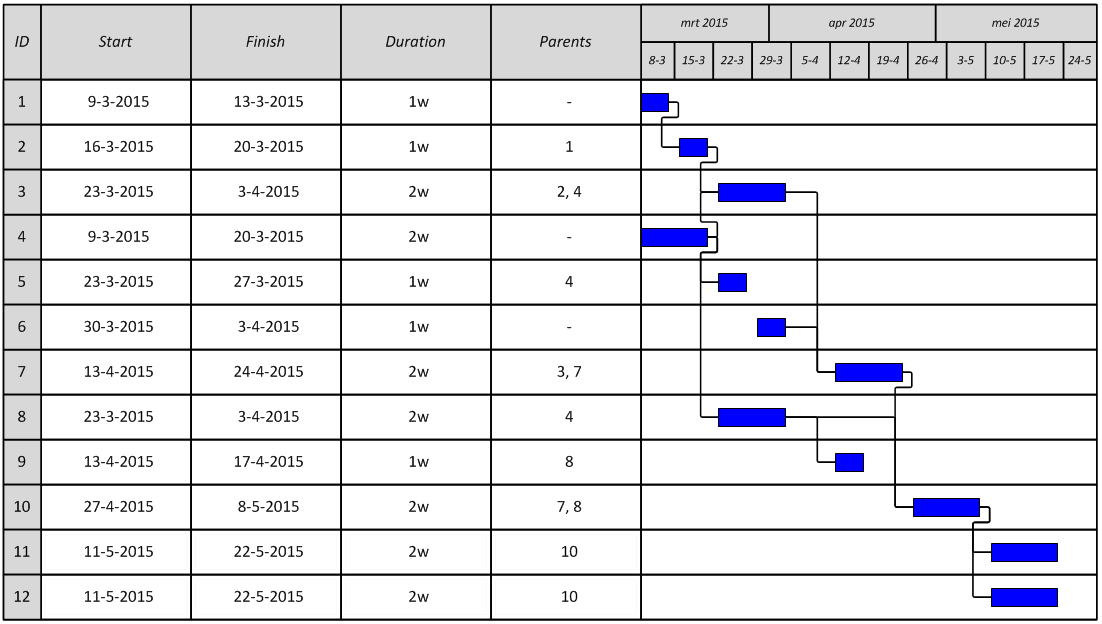
\includegraphics[scale=0.5]{Gantt}
\caption{Gantt chart showing the workpackage dependencies and the total planning}
\end{figure}

\section{Outcomes and Demonstration}

As a result of the project, a memorysize comparison will be made between the demonstrated data structure and the naive approach of storing one voxel grid per timeframe.
Also, it should be demonstrated that the scene can still be reconstructed at any point in time. Therefore, it is proposed to record a scene during the final presentation 
and demonstrate that a 3D model can be recovered at a time frame picked by the audience. Moreover, some prerecorded scenes are planned which allow for demonstration of specific aspects 
e.g. higly dynamic scenes, lengthier scenes, and fusing of a large amount of cameras.


%\vspace{1cm}
%\textbf{Instructions:}
%
%\begin{itemize}
%\item The document should not exceed two pages including the references.
%\item Please name the document \textbf{3DPhoto\_Proposal\_Surname1\_Surname2.pdf} and send it to Ya\u{g}{\i}z in an email titled \textbf{[3DPhoto] Project Proposal - Surname1 Surname2}, filling in your surnames.
%\end{itemize}

{%\singlespace
{\small
%\bibliography{refs}
\bibliographystyle{plain}}}




\end{document}